\documentclass{article}

\usepackage{graphicx}
\usepackage{amsmath}
\usepackage{mathtools}

\usepackage[utf8]{inputenc}
\usepackage[english]{babel}
\usepackage{mathrsfs,amsmath}
\usepackage{float}
\usepackage{subfig}


% Puts captions of tables on top
\floatstyle{plaintop}
\restylefloat{table}

% Puts captions in bold
\captionsetup{labelfont=bf}

\begin{document}

\begin{titlepage}
\begin{center}

\textsc{\LARGE Delft University of Technology}\\[1.5cm]
\textsc{ SC4045 Control for High Resolution Imaging}\\[0.5cm]

% Title
{\huge\bfseries Wavefront Reconstruction \\[0.4cm] }

% Author and supervisor
\begin{minipage}{0.4\textwidth}
\begin{flushleft} \large
\emph{Author:}\\
Jacco van der Spek \\
4002512 \\
Niels Tielen \\
4011147

\end{flushleft}
\end{minipage}
\begin{minipage}{0.4\textwidth}
\begin{flushright} \large
\emph{Supervisors:} \\
Prof. M. Verhagen \\
Phd. João P. Lopes e Silva  
\end{flushright}
\end{minipage}

\vfill
% Bottom of the page
{\large \today}
\end{center}
\end{titlepage}

\section*{Introduction}

In the previous part of this report, we already mentioned the first steps in the use of adaptive optics. First we described waverfront generating and wavefront sensing. In this chapter of the report, we take a closer look at the reconstruction of the wavefront. 

\section{Zonal Reconstruction}
In order to describe the gradient of the wavefront, we first take a look at a zonal reconstruction method. With zonal reconstruction, we split up the wavefront in zones. These zones can represent a regular grid of square or rectangular elements or some other local region such as a hexagonal or other shape. For Shack-Hartmann wavefront sensors, the type of sensor that is used, these zones are generally chosen to match the lenslets.

\subsection{reconstruction of wavefront slopes}
As can be seen in the part of the centroid algorithm, the relation between the slope of the wavefront and the wavefront phase can be defined as the following partial derivative:
$$ \sigma_x = \frac{\partial\phi(x,y)}{\partial x}$$ 
$$ \sigma_y = \frac{\partial\phi(x,y)}{\partial y}$$ 
In order to estimate the derivatives, we need to use a finite difference (FD) method. There are a number of different FD methods which depend on the sampling geometry. Some of these geometries are the Fried, Hudgin and Southwell geometries. We first start with a detailed explanation of the Fried geometry.

\subsection{Fried Geometry}
The Fried FD method calculates the average slope in one grid cell by using the four phase points. We first take a look at one part of the cell grid.
\begin{figure}[h!]
  \centering
%  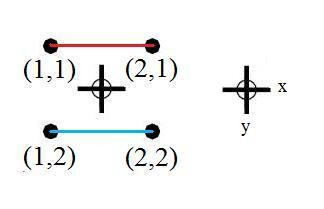
\includegraphics[scale=0.6]{figures/fried}
  \caption{slope approximation}
\end{figure}
\newpage
\noindent The goal is to calculate average of the both slopes. The first slope (in the x-direction) is given by the red line. We can easily see that this slope is given by:
$$ \sigma_{x,red} = \frac{\phi(2,1) - \phi(1,1)}{Dl} $$
where $Dl$ is the step between the 2 phase measurments, ussualy the size of the subapperature.
Now we do the same for the other slope:
$$ \sigma_{x,blue} = \frac{\phi(2,2) - \phi(1,2)}{Dl} $$
Now we take the average of these 2 slopes on then we know the slope of the wavefront in this zone (for x-direction).
$$ \sigma_x = \frac{\sigma_{x,red}+\sigma_{x,blue}}{2}$$
$$ \sigma_x = \frac{(\phi(2,1) - \phi(1,1))+(\phi(2,2) - \phi(1,2))}{2Dl}$$
From this example, we can derive a general method for calculating the slope. 
$$ \sigma_x = \frac{[(\phi(i+1,j)-\phi(i,j))+(\phi(i+1,j+1)-\phi(i,j+1)]}{2Dl} + n_x(i,j)$$
$$ \sigma_y = \frac{[(\phi(i,j+1)-\phi(i,j))+(\phi(i+1,j+1)-\phi(i+1,j)]}{2Dl} + n_y(i,j)$$
This is the Fried geometry model. Later in this chapter the Southwell and Hudgin geometries will be introduced, but for now we stick with the Fried geometry.  

\subsection{Creating the geometry matrix}
The next step is to take geometry model and structurize it in an ordery fashion. We structurize the model as followed:
$$ s = G\phi + n$$  
Here s is the vector containing the slopes, made by appending $[\sigma_x \sigma_y]^T$. $\phi$ is a vector filled with the phase points used define the slope and n is the noise. The equations used to link $\phi$ with $s$ can be found in the geometry matrix G. In our previous example we can derive the following G matrix:
$$ 
\begin{bmatrix}
\sigma_x \\
\sigma_y
\end{bmatrix} 
=
G
*
\begin{bmatrix}
\phi(1,1) \\
\phi(2,1) \\
\phi(1,2) \\
\phi(2,2) 
\end{bmatrix}
$$
Where, in this case, G is defined as:
$$
G
=
\frac{\alpha}{2Dl}
\begin{bmatrix}
-1 & 1 & -1 & 1 \\
-1 & -1 & 1 & 1 \\
\end{bmatrix}
$$

\subsection{Hudgin Geometries}
As mentioned before, there are many other geometries that can be used to generate a geometry matrix. Earlier we mentioned the Hudgin an Southwell geometry besides the Fried geometry. We first start to take a closer look at the Hudgin geometry.
\newline
\newline
Lets take a look at the way the Hudgin geometry is defined. First we start with an overview of the slopes and phase points.
\begin{figure}[h!]
  \centering
 % \includegraphics[scale=0.6]{figures/Hudgin}
  \caption{slope approximation, Hudgin}
\end{figure}
From this we can easily derive the slope approximation in x and y direction. These are given by the following equations:
$$ \sigma_x = \frac{\phi(2,1)-\phi(1,1)}{Dl}$$
$$ \sigma_y = \frac{\phi(1,2)-\phi(1,1)}{Dl}$$
From these equations we can derive the geometry matrix, just as we have done with the Fried geometry. But if we look closer to Figure 2, we see that slopes $\sigma_x$ and $\sigma_y$ aren`t defined in the same point, as with the Fried geometry. Due to our sensor, the Shack-Hartmann sensor, and it`s centroid algorithm, we only have the 2 slopes in the same point. As this geometry requires the slopes at 2 different pionts, we have to conclude that we cannot use the Hudgin geometry. But fortunatly, we can alter the Hudgin geometry slightly, and use it on a Shack-Hartmann snesor. This is called the `Modified` Hudgin geometry.
\newline
\newline
The Modified Hudgin geometry uses the same theory as the Hudgin geometry, but it makes it capable for being used in a Shack-Hartmann sensor. Let`s take a look at an overview of the slopes and phase points as they are used in the Modified Hudgin geometry.  
\newpage
\begin{figure}[h!]
  \centering
 % 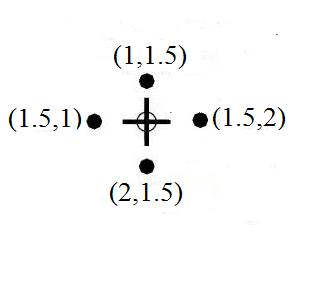
\includegraphics[scale=0.6]{figures/mod_hudgin}
  \caption{slope approximation, Modified Hudgin}
\end{figure}
\noindent Now we can see that we can use the slope information from the centroid algorithm to define four phase points to do the reconstruction. Now we can derive the equations that define the 2 slopes:
$$ \sigma_x = \frac{\phi(1.5,2)-\phi(1.5,1)}{Dl}$$
$$ \sigma_y = \frac{\phi(2,1.5)-\phi(1,1.5)}{Dl}$$
And just as we did with the Fried geometry, we can define a geometry matrix $G$:
$$ 
\begin{bmatrix}
\sigma_x \\
\sigma_y
\end{bmatrix} 
=
G
*
\begin{bmatrix}
\phi(1,1.5) \\
\phi(1.5,1) \\
\phi(1.5,2) \\
\phi(2,1.5) 
\end{bmatrix}
$$
Where, in this case, G is defined as:
$$
G
=
\frac{\alpha}{Dl}
\begin{bmatrix}
0 & -1 & 1 & 0 \\
-1 & 0 & 0 & 1 \\
\end{bmatrix}
$$


\end{document}
